\documentclass{beamer}

% $Header$
\usepackage{listings}
\usepackage{tcolorbox}
\usepackage{graphicx}
\usepackage{xcolor}
\usepackage{../shared/listings-rust}

\definecolor{codegreen}{rgb}{0,0.6,0}
\definecolor{codegray}{rgb}{0.5,0.5,0.5}
\definecolor{codepurple}{rgb}{0.58,0,0.82}
\definecolor{backcolour}{rgb}{0.95,0.95,0.92}

\lstdefinestyle{mystyle}{
    backgroundcolor=\color{backcolour},
    commentstyle=\color{codegreen},
    keywordstyle=\color{magenta},
    numberstyle=\tiny\color{codegray},
    stringstyle=\color{codepurple},
    basicstyle=\ttfamily\footnotesize,
    breakatwhitespace=false,
    breaklines=true,
    captionpos=b,
    keepspaces=true,
    numbers=left,
    numbersep=5pt,
    showspaces=false,
    showstringspaces=false,
    showtabs=false,
    tabsize=2
}

\lstset{style=mystyle, inputpath=src/, language=Rust}

\graphicspath{ {./media/} }

\newtcbox{\inlinecode}{nobeforeafter, tcbox raise base, boxrule=0mm, top=0mm, bottom=0mm, right=0mm, left=0mm}

% This file is a solution template for:

% - Talk at a conference/colloquium.
% - Talk length is about 20min.
% - Style is ornate.



% Copyright 2004 by Till Tantau <tantau@users.sourceforge.net>.
%
% In principle, this file can be redistributed and/or modified under
% the terms of the GNU Public License, version 2.
%
% However, this file is supposed to be a template to be modified
% for your own needs. For this reason, if you use this file as a
% template and not specifically distribute it as part of a another
% package/program, I grant the extra permission to freely copy and
% modify this file as you see fit and even to delete this copyright
% notice.

\mode<presentation>
{
  \usetheme{AnnArbor}
  % \usetheme{CambridgeUS}
  % or ...

  % \setbeamercovered{transparent}
  % or whatever (possibly just delete it)
}


\usepackage[english]{babel}
% or whatever

\usepackage[latin1]{inputenc}
% or whatever

\usepackage[T1]{fontenc}
% Or whatever. Note that the encoding and the font should match. If T1
% does not look nice, try deleting the line with the fontenc.

\title{Common Programming Task}
\subtitle{IEEE42069 Introduction to \ensuremath{\mathrm{Fe_{2}O_{3}}} / \ensuremath{\mathrm{Fe{(OH)}_{3}}}}

\author[]{Tan Hong Kai}
% - Give the names in the same order as the appear in the paper.
% - Use the \inst{?} command only if the authors have different
%   affiliation.

\institute[]{IEEE UNM}
% - Use the \inst command only if there are several affiliations.
% - Keep it simple, no one is interested in your street address.

\date[]{IEEE Workshop}
% - Either use conference name or its abbreviation.
% - Not really informative to the audience, more for people (including
%   yourself) who are reading the slides online

\subject{Programming}
% This is only inserted into the PDF information catalog. Can be left
% out.

% If you have a file called "university-logo-filename.xxx", where xxx
% is a graphic format that can be processed by latex or pdflatex,
% resp., then you can add a logo as follows:

\pgfdeclareimage[height=0.5cm]{university-logo}{../shared/Nottingham}
\logo{\pgfuseimage{university-logo}}


% If you wish to uncover everything in a step-wise fashion, uncomment
% the following command:
% \beamerdefaultoverlayspecification{<+->}

\hypersetup{backref,
     pdfpagemode=FullScreen,
     colorlinks=true}


\title{Installing Rust}

\begin{document}
\begin{frame}
  \titlepage{}
\end{frame}

\section{Setting Up Rust}
\subsection{Installing Rust}
\begin{frame}
  \frametitle{Installing rustup for Windows}
  \begin{enumerate}
    \item{Go To:

          \url{https://www.rust-lang.org/tools/install}}
    \pause{}
    \item{Download the relevant `rustup-init.exe' file (32-bit or 64-bit)}
    \pause{}
    \item{Install Visual Studio build tools if needed.

          \url{https://visualstudio.microsoft.com/downloads/}

          Work load to include when prompted:
          \begin{itemize}
            \item{'Desktop Development with C++'}
            \item{The Windows 10 or 11 SDK}
            \item{The English language pack component, along with any other language pack of your choosing}
          \end{itemize}
          }
  \end{enumerate}
\end{frame}


\begin{frame}
  \frametitle{Installing rustup for Windows}
  \begin{enumerate}
          \setcounter{enumi}{3}
    \item<+->{Adding Rust to \lstinline[backgroundcolor=backcolour]{PATH} Enviornment Variable (might not be needed)

          All rust tools are installed in \inlinecode{C:/Users/\emph{username}/.cargo/bin}
          }
          \begin{columns}[t]
              \begin{column}{.5\linewidth}
                \begin{enumerate}
                        \setcounter{enumii}{4}
                  \item<+->{Go to System Properties and click Enviornment Variables}
                        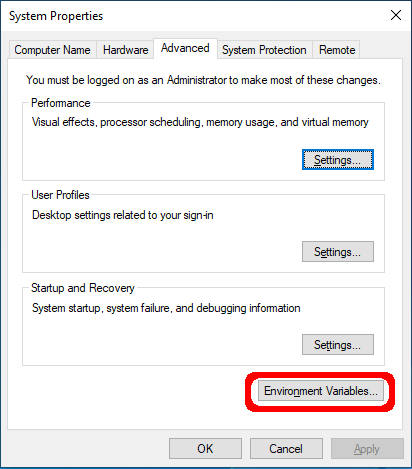
\includegraphics[height=5cm]{system_property.png}
                \end{enumerate}
              \end{column}
              \begin{column}{.5\linewidth}
                \begin{enumerate}
                        \setcounter{enumii}{5}
                  \item<+->{Add the respective PATH to it e.g.C:/Users/\emph{SUSKE}/.cargo/bin}
                        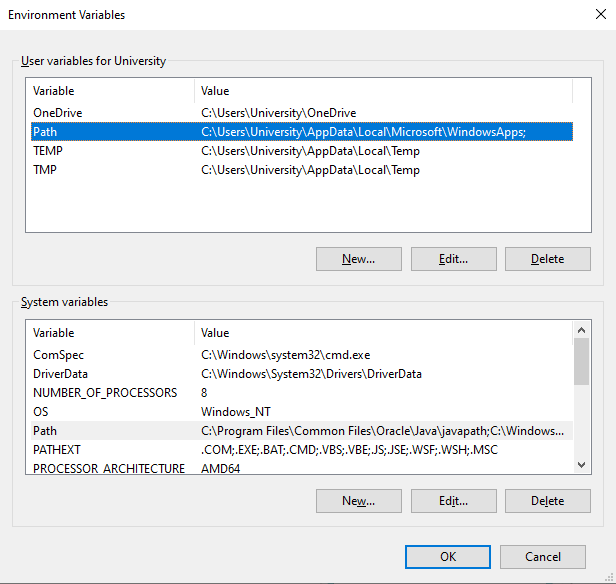
\includegraphics[height=5cm]{path.png}
                \end{enumerate}
              \end{column}
          \end{columns}
  \end{enumerate}
\end{frame}


\begin{frame}[fragile]
  \frametitle{Installing rustup for Unix Like (Linux/MacOS) Operating Systems}
  \begin{enumerate}
    \item{Open up a terminal}
    \item{Run:

\begin{semiverbatim}
\$ curl --proto '=https' --tlsv1.3 https://sh.rustup.rs -sSf
 | sh
\end{semiverbatim}
          }
    \item{Follow the instructions}
    \item{Making sure a linker is installed

          On MacOS:\@
\begin{semiverbatim}
\$ xcode-select --install
\end{semiverbatim}

          On Linux, follow distribution documentation instructions on installing GCC or Clang:

          On Ubuntu:
\begin{semiverbatim}
\$ sudo apt update \&\& sudo apt upgrade
\$ sudo apt install build-essential
\end{semiverbatim}
          }
  \end{enumerate}
\end{frame}

\begin{frame}[fragile]
  \frametitle{Testing Installation}

  To check whether Rust is installed correctly run in any CLI e.g. PowerShell and CMD on windows or terminal on Unix:
\begin{semiverbatim}
\$ rustc ---version
\end{semiverbatim}

  If the installation is successful, the output of the command should appear something like this:
\begin{semiverbatim}
rustc x.y.z (abcabcabc yyyy-mm-dd)
\end{semiverbatim}

  If it didn't work double check if the \inlinecode{PATH} variable is setup correctly.
\end{frame}

\subsection{Setting Up IDE/rust-analyzer}

% \begin{frame}{Outline}
  % \tableofcontents
  % You might wish to add the option [pausesections]
% \end{frame}

\section{Hello World}

\begin{frame}[fragile]
  \frametitle{Your First Rust Code}

  Here is a simple example of a Rust code that prints ``Hello World''
\begin{lstlisting}[language=Rust]
  fn main() {
    println!("Hello World");
  }
\end{lstlisting}

  The file extension of Rust source code file is \inlinecode{.rs}. Save this file as \inlinecode{hello\_world.rs}.

  The follow sections will guide you through the work flow of compiling and running Rust programs.
\end{frame}

\subsection{Using rustc}
\begin{frame}[fragile]{Compiling Using rustc}
  The \inlinecode{rustc} binary is the compiler of Rust. To compile the a Rust code simply run:

\begin{lstlisting}
$ rustc hello_world.rs
\end{lstlisting}

  A new binary file should be created with the same name as your source code file. In this case it is \inlinecode{hello\_world}. Now test out the binary.

\begin{lstlisting}
$ ./hello_world
Hello World
\end{lstlisting}

  \alert{Note:} If you are compiling on other operating systems the resultant binary might have extensions such as \inlinecode{.exe} on Windows. However, the resultant binary should still have the same behavior.
\end{frame}

\subsection{Using cargo}
\begin{frame}[fragile]
  \frametitle{Compiling Using Cargo}
  Normally Rust programmers will start new projects using cargo. Cargo is Rust's package manager like apt on Ubuntu/Debian. You can also use it to create your own package and build Rust code.
\begin{lstlisting}
$ cargo new hello_world
$ cd hello_world
$ cargo build
\end{lstlisting}

  The binary should be created in the path \inlinecode{target/debug/\emph{packagename}}. You can just run the built binary file or you can run it using cargo.

\begin{lstlisting}
$ cargo run
\end{lstlisting}

  \inlinecode{cargo run} will build the binary if any changes is made to the source code and run the resultant binary.
\end{frame}

\section{IDE Integration}
\begin{frame}[fragile]
  \frametitle{IDE}
  An Integrated Development Enviornment (IDE). In layman's term a fancy text editor that helps you code.

  \inlinecode{rust-analyzer} is a tool made by the Rust community to help with IDE integration. It speaks Language Server Protocol (LSP) that helps IDE and programming languages to communiticate with each other.

  Website Homepage: \url{https://rust-analyzer.github.io/}

  The rust-analyzer binary needs to be installed for most editor to interact with it (not needed for VS Code). The binary is available in \inlinecode{rustup}.
\begin{lstlisting}[language=bash]
$ rustup component add rust-analyzer
\end{lstlisting}

  \alert{Note:} It might not be installed in \inlinecode{.cargo/bin} directory. Please refer to \inlinecode{rust-analyzer} \href{https://rust-analyzer.github.io/manual.html}{manual} for more information.
\end{frame}

\subsection{Emacs}

\begin{frame}[fragile]{Rust mode \& Rustic mode}
  \inlinecode{rust-mode} is a mode created to help write Rust code in Emacs. \inlinecode{rustic-mode} is a superset of \inlinecode{rust-mode}, it provides additional features to \inlinecode{rust-mode} such as cargo popup and automatic LSP configuration.

  To install paste this into your \inlinecode{init.el}:
\begin{lstlisting}[language=Lisp]
(require 'package)
(setq package-archives '(("melpa" . "http://melpa.org/packages/")
                         ("gnu" . "http://elpa.gnu.org/packages/")))
(package-initialize)
(package-refresh-contents)
(use-package rustic)
\end{lstlisting}

  \alert{Note:} The \inlinecode{use-pacakge} and \inlinecode{rustic} package needs to be \href{https://www.emacswiki.org/emacs/InstallingPackages}{installed}.
\end{frame}

\begin{frame}
\frametitle[Rustic Keybindings]{Rustic Keybindings/Commands}
\inlinecode{C-c C-c C-u}: Compile your current project using cargo.

\inlinecode{C-c C-c C-r}: Runs \inlinecode{cargo run}.

\inlinecode{C-c C-c a}: Adds a new crate to the project's Cargo.toml

\inlinecode{C-c C-c r}: Removes a crate from the project's Cargo.toml

\inlinecode{C-c C-c C-f}: Formats your current buffer using \inlinecode{rustfmt}.

\inlinecode{C-c C-c d}: Generates documentation for the current cargo project.

\inlinecode{C-c C-c C-t}: Runs \inlinecode{cargo test} for the current project. (Running Tests)

\inlinecode{C-c C-p}: Shows a popup window that runs commands.

More commands are documented in rustic \href{https://github.com/brotzeit/rustic}{GitHub README.md}.
\end{frame}

\subsection{VS Code (Cringe)}
\begin{frame}
  \frametitle{Visual Studio Code Plugin (Cringe)}
  The IDE integration for VS Code is done by installing the \inlinecode{rust-analyzer} plugin in the \href{https://marketplace.visualstudio.com}{Visual Studio Code marketplace}.
  \begin{enumerate}
    \item<+->{Go to the extensions tab (Ctrl + Shift + X)}
    \item<+->{Search for rust-analyzer}
    \item<+->{Hit install on the rust-analyzer extension}
  \end{enumerate}

  For more information on how to install extenstions in VS Code, visit the VS Code \href{https://code.visualstudio.com/docs/editor/extension-marketplace}{documentation}.
\end{frame}

% All of the following is optional and typically not needed.
\appendix
\section<presentation>*{\appendixname}
\subsection<presentation>*{Additional Resources}
\begin{frame}[allowframebreaks]
  \frametitle<presentation>{Additional Resources}
  \href{https://doc.rust-lang.org/stable/book}{The Rust Programming Language Book}

  \href{https://github.com/rust-lang/rustlings}{Rustlings}

  \href{https://doc.rust-lang.org/stable/rust-by-example/index.html}{Rust By Example}

  \href{https://www.rust-lang.org/tools}{Rust Tools}

  \href{https://play.rust-lang.org/}{Rust Playground}

  Rust Documentation
  \begin{itemize}
    \item{Local Installation

          \inlinecode{\$ rustup doc}}
    \item{\href{https://doc.rust-lang.org/stable/}{Online Documentation}}
  \end{itemize}
\end{frame}

\subsection<presentation>*{Additional Resources}
\begin{frame}
  \frametitle{IDE With Top Class Support}
  \begin{itemize}
    \item{Emacs}
    \item{VS Code}
    \item{Vim}
    \item{Sublime Text}
    \item{Atom}
    \item{Intellij Idea}
    \item{Eclipse}
    \item{Geany}
  \end{itemize}
\end{frame}

\end{document}
